\begin{name}
	{\tenchude}{\tendethi}{LỚP TOÁN THẦY PHÁT}{\thoigian}
\end{name}
\setcounter{ex}{0}\setcounter{bt}{0}
\Opensolutionfile{ans}[ans/ans-2-TT-11-SGD-HungYen-23]

\begin{ex}%[Thi thử tốt nghiệp - SGD Hưng Yên - 23]%[Lê Văn Toàn - EX6-2023]%[2D3Y1-1]
	Họ nguyên hàm của hàm số $f(x)=2^x$ là
	\choice
	{$2^x\cdot \ln 2+C$}
	{$\dfrac{\ln 2}{2^x}+C$}
	{\True $\dfrac{2^x}{\ln 2}+C$}
	{$x\cdot 2^x\cdot \ln 2+C$}
	\loigiai{
		Ta có $\displaystyle\int\limits 2^x\mathrm{\,d}x=\dfrac{2^x}{\ln 2}+C$.
	}
\end{ex}


\begin{ex}%[Thi thử tốt nghiệp - SGD Hưng Yên - 23]%[Lê Văn Toàn - EX6-2023]%[2D3Y1-1]
	Họ tất cả các nguyên hàm của hàm số $f(x)=2x-\sin x$ trên tập $\mathbb{R}$ là
	\choice
	{\True $x^2+\cos x+C$}
	{$2x^2-\cos x+C$}
	{$x^2-\cos x+C$}
	{$2x^2+\cos x+C$}
	\loigiai{
		Ta có $\displaystyle\int\limits (2x-\sin x)\mathrm{\,d}x=x^2+\cos x+C$.
	}
\end{ex}


\begin{ex}%[Thi thử tốt nghiệp - SGD Hưng Yên - 23]%[Lê Văn Toàn - EX6-2023]%[2D1Y5-4]
	\immini{
		Cho hàm số $y=\dfrac{ax+b}{cx+d}$ có đồ thị là đường cong như hình dưới đây. Tìm tọa độ giao điểm của đồ thị hàm số đã cho và trục tung.
		\choice
		{$(0;-1)$}
		{\True $(0;2)$}
		{$(2;0)$}
		{$(-1;0)$}
	}
	{
		\begin{tikzpicture}[scale=.6, font=\footnotesize, line join=round, line cap=round, >=stealth]
			\draw[->] (-5.1,0)--(4,0) node[above left] {$x$};
			\draw[->] (0,-5.1)--(0,4) node[below right] {$y$};
			\draw (0,0) node [below right] {$O$};
			\foreach \x in {2}
			\draw[thin] (\x,1pt)--(\x,-1pt) node [above] {$\x$};
			\foreach \x in {-1}
			\draw[thin] (\x,1pt)--(\x,-1pt) node [above left] {$\x$};
			\foreach \y in {-1}
			\draw[thin] (1pt,\y)--(-1pt,\y) node [below right] {$\y$};
			\foreach \y in {2}
			\draw[thin] (1pt,\y)--(-1pt,\y) node [right] {$\y$};
			\draw[thin] (-5,-1)--(4,-1);
			\begin{scope}
				\clip (-5,-5) rectangle (4,4);
				\draw[samples=200,domain=-5:4,smooth,variable=\x] plot (\x,{(-2*(\x)+4)/(2*(\x)+2)});
			\end{scope}
		\end{tikzpicture}
	}
	\loigiai{
		Dựa vào đồ thị ta thấy đồ thị hàm số giao với trục tung tại $(0;2)$.
	}
\end{ex}


\begin{ex}%[Thi thử tốt nghiệp - SGD Hưng Yên - 23]%[Lê Văn Toàn - EX6-2023]%[2D4Y1-1]
	Trong KG $Oxyz$, cho mặt phẳng $(P) \colon x+y+z-3=0$. Điểm nào sau đây không thuộc $(P)$?
	\choice
	{$F(3;2;-2)$}
	{\True $E(1;0;1)$}
	{$N(1;0;2)$}
	{$M(0;1;2)$}
	\loigiai{
		Xét điểm $E(1;0;1)$ ta có $1+0+1-3=-1$. Do đó, điểm $E(1;0;1)$ không thuộc mặt phẳng $(P)$.
	}
\end{ex}


\begin{ex}%[Thi thử tốt nghiệp - SGD Hưng Yên - 23]%[Lê Văn Toàn - EX6-2023]%[2D4Y1-1]
	Tìm phần ảo của số phức $z=2+\pi i$.
	\choice
	{$2$}
	{$-2$}
	{$-\pi$}
	{\True $\pi$}
	\loigiai{
		Số phức $z=2+\pi i$ có phần ảo là $\pi$.
	}
\end{ex}


\begin{ex}%[Thi thử tốt nghiệp - SGD Hưng Yên - 23]%[Lê Văn Toàn - EX6-2023]%[2H1Y3-2]
	Thể tích khối lăng trụ có diện tích đáy $B$ và chiều cao $h$ là
	\choice
	{$\dfrac{1}{3}Bh$}
	{$\dfrac{4}{3}Bh$}
	{$3Bh$}
	{\True $Bh$}
	\loigiai{
		Thể tích khối lăng trụ tính theo công thức $V=Bh$.
	}
\end{ex}


\begin{ex}%[Thi thử tốt nghiệp - SGD Hưng Yên - 23]%[Lê Văn Toàn - EX6-2023]%[2D4Y2-2]
	Phần thực của số phức $z=(3-4i)-(2+6i)$ bằng
	\choice
	{$9$}
	{$5$}
	{$-1$}
	{\True $1$}
	\loigiai{
		Ta có $z=(3-4i)-(2+6i)=1-10i$.\\
		Vậy phần thực của $z$ là $1$.
	}
\end{ex}


\begin{ex}%[Thi thử tốt nghiệp - SGD Hưng Yên - 23]%[Lê Văn Toàn - EX6-2023]%[2D2Y6-1]
	Tập nghiệm của bất phương trình $\log _2x>1$ là
	\choice
	{$(-\infty;2)$}
	{$(-\infty;0)$}
	{$(0;+\infty)$}
	{\True $(2;+\infty)$}
	\loigiai{
		Ta có $\log _2x>1 \Leftrightarrow x>2$.
	}
\end{ex}


\begin{ex}%[Thi thử tốt nghiệp - SGD Hưng Yên - 23]%[Lê Văn Toàn - EX6-2023]%[2D3Y1-1]
	Họ các nguyên hàm của hàm số $y=\mathrm{e}^x-2x$ là
	\choice
	{$\mathrm{e}^x-2x^2+C$}
	{$\mathrm{e}^x-2+C$}
	{\True $\mathrm{e}^x-x^2+C$}
	{$\dfrac{1}{x+1}\mathrm{e}^{x+1}-x^2+C$}
	\loigiai{
		Ta có $\displaystyle\int\limits (\mathrm{e}^x-2 x)\mathrm{\,d}x=\mathrm{e}^x-x^2+C$.
	}
\end{ex}


\begin{ex}%[Thi thử tốt nghiệp - SGD Hưng Yên - 23]%[Lê Văn Toàn - EX6-2023]%[2D4Y1-1]
	Cho số phức $z=2-3i$. Tính mô-đun của số phức $z$
	\choice
	{\True $\vert z\vert=\sqrt{13}$}
	{$\vert z\vert=1$}
	{$\vert z\vert=3\sqrt{3}$}
	{$\vert z\vert=\sqrt{5}$}
	\loigiai{
		Ta có $\vert z \vert=\sqrt{2^2+(-3)^2}=\sqrt{13}$.
	}
\end{ex}


\begin{ex}%[Thi thử tốt nghiệp - SGD Hưng Yên - 23]%[Lê Văn Toàn - EX6-2023]%[2H3Y1-3]
	Trong KG $Oxyz$, cho mặt cầu có phương trình $(x-4)^2+(y+2)^2+(z-5)^2=9$. Tìm tọa độ tâm $I$ và bán kính $R$ của mặt cầu đó.
	\choice
	{$I(-4;2;-5)$; $R=9$}
	{\True $I(4;-2;5)$; $R=3$}
	{$I(4;-2;5)$; $R=9$}
	{$I(-4;2;-5)$; $R=3$}
	\loigiai{
		Phương trình mặt cầu $(x-4)^2+(y+2)^2+(z-5)^2=9$ có tâm $I(4;-2;5)$ và bán kính $R=\sqrt{9}=3$.
	}
\end{ex}


\begin{ex}%[Thi thử tốt nghiệp - SGD Hưng Yên - 23]%[Lê Văn Toàn - EX6-2023]%[2H3Y2-2]
	Trong KG $Oxyz$, cho mặt phẳng $(\alpha) \colon 2x-3y+z-5=0$. Véc-tơ nào dưới đây là một véc-tơ pháp tuyến của $(\alpha)$?
	\choice
	{\True $\overrightarrow{n}_3=(2;-3;1)$}
	{$\overrightarrow{n}_1=(2;3;1)$}
	{$\overrightarrow{n}_2=(2;3;-1)$}
	{$\overrightarrow{n}_4=(-2;3;1)$}
	\loigiai{
		Mặt phẳng $(\alpha) \colon 2x-3y+z-5=0$ có một véc-tơ pháp tuyến là $\overrightarrow{n}_3=(2;-3;1)$.
	}
\end{ex}


\begin{ex}%[Thi thử tốt nghiệp - SGD Hưng Yên - 23]%[Lê Văn Toàn - EX6-2023]%[2D1Y1-2]
	Cho hàm số $y=f(x)$ có bảng biến thiên như sau
	\begin{center}
		
\begin{tikzpicture}
			\tkzTabInit[espcl=2.5,lgt=1.5]
			{$x$/0.7,$y'$/0.7,$y$/2.1}
			{$-\infty$,$-1$,0,$1$,$+\infty$}
			\tkzTabLine{,-,0,+,0,-,0,+}
			\tkzTabVar{+/$+\infty$,-/$0$,+/$5$,-/$0$,+/$+\infty$}
		\end{tikzpicture}
	\end{center}
	Hàm số $y=f(x)$ nghịch biến trên khoảng nào dưới đây?
	\choice
	{$(-\infty;0)$}
	{\True $(-\infty;-2)$}
	{$(-1;0)$}
	{$(0;+\infty)$}
	\loigiai{
		Dựa vào bảng biến thiên ta thấy hàm số nghịch biến trên khoảng $(-\infty;-1)$ nên nghịch biến trên khoảng $(-\infty;-2)$.
	}
\end{ex}


\begin{ex}%[Thi thử tốt nghiệp - SGD Hưng Yên - 23]%[Lê Văn Toàn - EX6-2023]%[2D2Y4-1]
	Điều kiện xác định của hàm số $y=\log _2(x+3)$ là
	\choice
	{$x\leq-3$}
	{$x<-3$}
	{$x\geq-3$}
	{\True $x>-3$}
	\loigiai{
		Hàm số $y=\log _2(x+3)$ xác định khi và chỉ khi $x+3>0 \Leftrightarrow x>-3$.
	}
\end{ex}


\begin{ex}%[Thi thử tốt nghiệp - SGD Hưng Yên - 23]%[Lê Văn Toàn - EX6-2023]%[2D1Y2-2]
	\immini{
		Cho hàm số bậc ba $y=f(x)$ có đồ thị là đường cong trong hình bên.
		Số điểm cực trị của hàm số đã cho là
		\choice
		{$3$}
		{$1$}
		{$0$}
		{\True $2$}
	}
	{
		\begin{tikzpicture}[scale=0.8, font=\footnotesize, line join=round, line cap=round, >=stealth]
			\draw[->] (-2.5,0)--(2.5,0) node[below left] {$x$};
			\draw[->] (0,-2.5)--(0,3) node[below left] {$y$};
			\draw (0,0) node [below left] {$O$};
			\foreach \x in {1}
			\draw[thin] (\x,1pt)--(\x,-1pt) node [below] {$\x$};
			\foreach \x in {-1}
			\draw[thin] (\x,1pt)--(\x,-1pt) node [above] {$\x$};
			\foreach \y in {2}
			\draw[thin] (1pt,\y)--(-1pt,\y) node [left] {$\y$};
			\foreach \y in {-2}
			\draw[thin] (1pt,\y)--(-1pt,\y) node [right] {$\y$};
			\draw[dashed,thin](1,0)--(1,2)--(0,2);
			\draw[dashed,thin](-1,0)--(-1,-2)--(0,-2);
			\begin{scope}
				\clip (-3,-3) rectangle (3,3);
				\draw[samples=200,domain=-2:2,smooth,variable=\x] plot (\x,{-1*((\x)^3)+0*((\x)^2)+3*(\x)+0});
			\end{scope}
		\end{tikzpicture}
	}
	\loigiai{
		Dựa vào đồ thị ta thấy đồ thị có $2$ điểm cực trị.
	}
\end{ex}


\begin{ex}%[Thi thử tốt nghiệp - SGD Hưng Yên - 23]%[Lê Văn Toàn - EX6-2023]%[2H2Y1-2]
	Cho hình trụ có bán kính đáy $R=8$ và độ dài đường sinh $\ell=3$. Diện tích xung quanh của hình trụ bằng
	\choice
	{$64\pi$}
	{$24\pi$}
	{\True $48\pi$}
	{$192\pi$}
	\loigiai{
		Diện tích xung quanh của hình trụ $S_\text{xq}=2\pi R \ell=2\pi \cdot 8 \cdot 3=48 \pi$.
	}
\end{ex}


\begin{ex}%[Thi thử tốt nghiệp - SGD Hưng Yên - 23]%[Lê Văn Toàn - EX6-2023]%[2D1Y4-1]
	Cho hàm số $y=f(x)$ có bảng biến thiên như sau
	\begin{center}
		
\begin{tikzpicture}[>=stealth]
			\tkzTabInit[nocadre=false,lgt=1,espcl=2,deltacl=0.5]
			{$x$/.7 ,$y'$/.7,$y$/2}
			{$-\infty$ , $0$, $3$, $+\infty$}
			\tkzTabLine{ ,-,d,-,$0$,  + , }
			\tkzTabVar{+/$-1$ ,-D+/$-\infty$/$2$ , -/$-3$,+/$3$,}
		\end{tikzpicture}
	\end{center}
	Số tiệm cận ngang của đồ thị hàm số đã cho là
	\choice
	{$4$}
	{$3$}
	{$1$}
	{\True $2$}
	\loigiai{
		Dựa vào bảng biến thiên ta thấy $\lim\limits_{x \to -\infty}y=-1$ và $\lim\limits_{x \to +\infty}y=3$.\\
		Do đó đồ thị có $2$ tiệm cận ngang là $y=-1$ và $y=3$.
	}
\end{ex}


\begin{ex}%[Thi thử tốt nghiệp - SGD Hưng Yên - 23]%[Lê Văn Toàn - EX6-2023]%[2D1Y3-2]
	Hàm số $y=g(x)$ có bảng biến thiên như hình sau
	\begin{center}
		\begin{tikzpicture}[>=stealth]
			\tkzTabInit[nocadre=false,lgt=1,espcl=3,deltacl=0.5]{$x$/.7 ,$g'(x)$/.7,$g(x)$/2}
			{$-\infty$, $0$, $1$ , $+\infty$}
			\tkzTabLine{,,,- , $0$,+}
			\fill[pattern=north east lines] (T11) rectangle ([xshift=-2mm]N23);
			\draw[->] ([xshift=5mm,yshift=16mm]N23) node[left]{$1$}--([xshift=-2.5mm,yshift=-16mm]N32) node[right]{$-2$};
			\draw[->] ([xshift=5mm,yshift=-16mm]N32)--([xshift=-4mm,yshift=16mm]N43) node[right]{$+\infty$};
		\end{tikzpicture}
	\end{center}
	Giá trị nhỏ nhất của hàm số trên khoảng $(0;+\infty)$ là
	\choice
	{$0$}
	{\True $-2$}
	{$-1$}
	{$1$}
	\loigiai{
		Dựa vào bảng biến thiên giá trị nhỏ nhất của hàm số trên khoảng $(0;+\infty)$ là	$-2$.
	}
\end{ex}


\begin{ex}%[Thi thử tốt nghiệp - SGD Hưng Yên - 23]%[Lê Văn Toàn - EX6-2023]%[1D2Y2-1]
	Lớp $12A1$ có $45$ học sinh. Có bao nhiêu cách chọn ra $5$ học sinh trong lớp $12A1$ tham gia lao động?
	\choice
	{$45$}
	{$\mathrm{A}_{40}^5$}
	{$\mathrm{P}_5$}
	{\True $\mathrm{C}_{45}^5$}
	\loigiai{
		Số cách chọn $5$ học sinh trong lớp $12A1$ có $45$ học sinh là $\mathrm{C}_{45}^5$.
	}
\end{ex}


\begin{ex}%[Thi thử tốt nghiệp - SGD Hưng Yên - 23]%[Lê Văn Toàn - EX6-2023]%[2H1Y2-2]
	Có bao nhiêu loại khối đa diện đều?
	\choice
	{$6$}
	{$3$}
	{$4$}
	{\True $5$}
	\loigiai{
		Có tất cả $5$ khối đa diện đều là loại $\{3,3\}$, $\{4,3\}$, $\{3,4\}$, $\{5,3\}$, $\{3,5\}$.
	}
\end{ex}


\begin{ex}%[Thi thử tốt nghiệp - SGD Hưng Yên - 23]%[Lê Văn Toàn - EX6-2023]%[1D3Y4-3]
	Cho cấp số nhân $\left(u_n\right)$ với $u_1=3$ và $u_2=-6$. Công bội $q$ của cấp số nhân đã cho là
	\choice
	{$q=-\dfrac{1}{2}$}
	{$q=-9$}
	{\True $q=-3$}
	{$q=-2$}
	\loigiai{
		Ta có $u_2=u_1 \cdot q \Rightarrow q=\dfrac{u_2}{u_1}=\dfrac{-6}{2}=-3$.
	}
\end{ex}


\begin{ex}%[Thi thử tốt nghiệp - SGD Hưng Yên - 23]%[Lê Văn Toàn - EX6-2023]%[2H3Y1-1]
	Trong KG $Oxyz$, cho hai điểm $A(3;-2;3)$ và $B(-1;2;5)$. Tìm tọa độ trung điểm $I$ của đoạn thẳng $AB$.
	\choice
	{$I(2;0;8)$}
	{$I(2;-2;-1)$}
	{$I(-2;2;1)$}
	{\True $I(1;0;4)$}
	\loigiai{
		Do $I$ là trung điểm nên ta có $\heva{&x_I=\dfrac{x_A+x_B}{2}=\dfrac{3-1}{2}=1\\&y_I=\dfrac{y_A+y_B}{2}=\dfrac{-2+2}{2}=0\\&z_I=\dfrac{z_A+z_B}{2}=\dfrac{3+5}{2}=4}$. Vậy $I(1;0;4)$.
	}
\end{ex}


\begin{ex}%[Thi thử tốt nghiệp - SGD Hưng Yên - 23]%[Lê Văn Toàn - EX6-2023]%[2H1B3-2]
	Cho hình chóp $S.ABCD$ có đáy $ABCD$ là hình vuông cạnh $2a$ và $SA$ vuông góc với đáy. Góc giữa $SC$ và đáy bằng $45^\circ$. Thể tích khối chóp $S.ABCD$ bằng
	\choice
	{\True $\dfrac{8a^3\sqrt{2}}{3}$}
	{$8a^3\sqrt{2}$}
	{$8a^3\sqrt{3}$}
	{$\dfrac{8a^3\sqrt{3}}{3}$}
	\loigiai{
		\immini{
			Ta có $(SC,(ABCD))=(SC,AC)=\widehat{SCA}=45^\circ$.\\
			Suy ra $\triangle SAC$ vuông cân tại $A \Rightarrow SA=AC=2a\sqrt{2}$.\\
			Vậy $V=\dfrac{1}{3}4a^2\cdot 2a\sqrt{2}=\dfrac{8a^3\sqrt{2}}{3}$.
		}
		{
			\begin{tikzpicture}[scale=0.45, font=\footnotesize, line join=round, line cap=round, >=stealth]
				\coordinate (A) at (0,0);
				\coordinate (B) at (-2,-3);
				\coordinate (D) at (7,0);
				\coordinate (C) at ($(B)+(D)-(A)$);
				\coordinate (S) at ($(A)+(0,5)$);
				\draw(S)--(B) (S)--(C) (S)--(D) (B)--(C)--(D);
				\draw[dashed,thin](S)--(A) (A)--(B) (A)--(D) (A)--(C);
				\draw pic[draw,angle radius=0.5cm]{angle=S--C--A};
				\pic[draw,thin,angle radius=2mm] {right angle = S--A--D} pic[draw,thin,angle radius=2mm] {right angle = S--A--B};
				\foreach \i/\g in {S/90,A/-90,B/-90,C/-90,D/0}{\draw[fill=black](\i) circle (1pt) ($(\i)+(\g:3mm)$) node[scale=1]{$\i$};}
			\end{tikzpicture}
		}
	}
\end{ex}


\begin{ex}%[Thi thử tốt nghiệp - SGD Hưng Yên - 23]%[Lê Văn Toàn - EX6-2023]%[1D2B5-2]
	Gieo đồng tiền $3$ lần. Xác suất để mặt ngửa xuất hiện ít nhất $1$ lần bằng
	\choice
	{$\dfrac{3}{8}$}
	{$\dfrac{3}{4}$}
	{$\dfrac{1}{8}$}
	{\True $\dfrac{7}{8}$}
	\loigiai{
		Ta có $n(\Omega)=2^3=8$.\\
		Gọi $\overline{A}$ là biến cố mặt ngửa không xuất hiện lần nào, $n(\overline{A})=1$.\\
		Vậy $\mathrm{P}(A)=1-\mathrm{P}(\overline{A})=1-\dfrac{n(\overline{A})}{n(\Omega)}=1-\dfrac{1}{8}=\dfrac{7}{8}$.
	}
\end{ex}


\begin{ex}%[Thi thử tốt nghiệp - SGD Hưng Yên - 23]%[Lê Văn Toàn - EX6-2023]%[2D1B2-1]
	Cho hàm số $y=f(x)$ có đạo hàm $f'(x)=(x-1)^2(x+1)(x-2)$. Hàm số $f(x)$ có bao nhiêu điểm cực trị?
	\choice
	{$3$}
	{$1$}
	{$0$}
	{\True $2$}
	\loigiai{
		Ta có $f'(x)=0 \Rightarrow (x-1)^2(x+1)(x-2)=0 \Leftrightarrow \hoac{&x=1\ (\text{bội chẵn})\\&x=-1\\&x=2.}$\\
		Bảng xét dấu
		\begin{center}
			
\begin{tikzpicture}
				\tkzTabInit[deltacl=0.5,espcl=2.5,lgt=2]
				{$x$/0.6,$f'(x)$/0.6}
				{$-\infty$,$-1$,$1$,$2$,$+\infty$}
				\tkzTabLine{,+,0,-,0,-,0,+,}
			\end{tikzpicture}
		\end{center}
		Dựa vào bảng xét dấu đạo hàm ta thấy hàm số có $2$ cực trị.
	}
\end{ex}


\begin{ex}%[Thi thử tốt nghiệp - SGD Hưng Yên - 23]%[Lê Văn Toàn - EX6-2023]%[2D2B3-1]
	Với $a$ là số thực dương tuỳ ý, $\log \left(\dfrac{10}{a^3}\right)$ bằng
	\choice
	{$1+3\log a$}
	{\True $1-3\log a$}
	{$1-\dfrac{1}{3}\log a$}
	{$1+\dfrac{1}{3}\log a$}
	\loigiai{
		Với $a$ là số thực dương tuỳ ý, ta có $\log \left(\dfrac{10}{a^3}\right)=\log 10-\log a^3=1-3\log a$.
	}
\end{ex}


\begin{ex}%[Thi thử tốt nghiệp - SGD Hưng Yên - 23]%[Lê Văn Toàn - EX6-2023]%[2H3B3-2]
	Viết PTTS của đường thẳng $d$ đi qua $A(1;2;3)$ và vuông góc với mặt phẳng $(\alpha)$ có phương trình $x-2y+z+1=0$.
	\choice
	{\True $\heva{&x=1+t \\ &y=2-2t \\ &z=3+t}$}
	{$\heva{&x=1+t \\ &y=2-2t \\ &z=3-t}$}
	{$\heva{&x=1+t \\ &y=-2+2t \\ &z=1+3t}$}
	{$\heva{&x=1+t \\ &y=-2+2t \\ &z=-1+3t}$}
	\loigiai{
		Vì đường thẳng $d$ qua $A(1;2;3)$ và vuông góc với mặt phẳng $(\alpha)$ nên $d$ có một véc-tơ chỉ phương là $\overrightarrow{u}=(1;-2;1)$.\\
		Vậy $d$ có PTTS là $\heva{&x=1+t \\ &y=2-2t \\ &z=3+t.}$
	}
\end{ex}


\begin{ex}%[Thi thử tốt nghiệp - SGD Hưng Yên - 23]%[Lê Văn Toàn - EX6-2023]%[2D3B2-1]
	Cho hàm số $f(x)$ liên tục trên $R$ và $\displaystyle\int\limits_0^4f(x) \mathrm{\,d}x=8$, $\displaystyle\int\limits_3^4f(x) \mathrm{\,d}x=2$. Tích phân $\displaystyle\int\limits_0^3f(x) \mathrm{\,d}x$ bằng
	\choice
	{\True $6$}
	{$10$}
	{$-6$}
	{$4$}
	\loigiai{
		Ta có $\displaystyle\int\limits_0^4f(x) \mathrm{\,d}x=\displaystyle\int\limits_0^3f(x) \mathrm{\,d}x+\displaystyle\int\limits_3^4f(x) \mathrm{\,d}x \Rightarrow \displaystyle\int\limits_0^3f(x) \mathrm{\,d}x=\displaystyle\int\limits_0^4f(x) \mathrm{\,d}x-\displaystyle\int\limits_3^4f(x) \mathrm{\,d}x=8-2=6$.
	}
\end{ex}


\begin{ex}%[Thi thử tốt nghiệp - SGD Hưng Yên - 23]%[Lê Văn Toàn - EX6-2023]%[2D1B5-4]
	Biết đồ thị hàm số $y=x^3+3x+4$ cắt đường thẳng $y=x+4$ tại điểm $M(a;b)$. Tính $a+b$.
	\choice
	{$-2$}
	{$3$}
	{\True $4$}
	{$0$}
	\loigiai{
		Phương trình hoành độ giao điểm của hai đồ thị là
		$$x^3+3x+4=x+4 \Leftrightarrow x^3+2x=0 \Leftrightarrow x=0.$$
		Khi đó $M(0;4)$. Vậy $a+b=0+4=4$.
	}
\end{ex}


\begin{ex}%[Thi thử tốt nghiệp - SGD Hưng Yên - 23]%[Lê Văn Toàn - EX6-2023]%[2D2B5-1]
	Tập nghiệm của phương trình $2^{x^2-x+2}=4$ là
	\choice
	{$S=\{0\}$}
	{$S=\{-1;0\}$}
	{$S=\{-1\}$}
	{\True $S=\{0;1\}$}
	\loigiai{
		Ta có $2^{x^2-x+2}=4 \Leftrightarrow 2^{x^2-x+2}=2^2 \Leftrightarrow x^2-x+2=2 \Leftrightarrow \hoac{&x=0\\&x=1.}$
	}
\end{ex}


\begin{ex}%[Thi thử tốt nghiệp - SGD Hưng Yên - 23]%[Lê Văn Toàn - EX6-2023]%[2H3B3-3]
	Tìm hình chiếu của điểm $M(2;0;1)$ trên mặt phẳng $(\alpha) \colon x+y+z=0$.
	\choice
	{$M'(2;0;1)$}
	{$M'(4;2;3)$}
	{$M'(3;1;2)$}
	{\True $M'(1;-1;0)$}
	\loigiai{
		Gọi $\Delta$ là đường thẳng qua $M$ và vuông góc với mặt phẳng $(\alpha)$.\\
		Đường thẳng $\Delta$ có véc-tơ chỉ phương $\overrightarrow{u}_\Delta=(1;1;1)$ và đi qua điểm $M(2;0;1)$ có PTTS là $\heva{&x=2+t\\&y=t\\&z=1+t.}$\\
		Giao điểm $M'=\Delta\cap (\alpha)$ là hình chiếu. Suy ra $(2+t)+t+(1+t)=0 \Leftrightarrow 3t+3=0 \Leftrightarrow t=-1 \Rightarrow H(1;-1;0)$.
	}
\end{ex}


\begin{ex}%[Thi thử tốt nghiệp - SGD Hưng Yên - 23]%[Lê Văn Toàn - EX6-2023]%[2D3B3-3]
	Thể tích khối tròn xoay khi quay hình phẳng $(H)$ xác định bởi các đường $y=\dfrac{1}{3}x^3-x^2$ và $y=0$ quanh trục $Ox$ là
	\choice
	{$\dfrac{81}{35}$}
	{$\dfrac{71}{35}$}
	{$\dfrac{71\pi}{35}$}
	{\True $\dfrac{81\pi}{35}$}
	\loigiai{
		Phương trình hoành độ giao điểm $\dfrac{1}{3}x^3-x^2=0 \Leftrightarrow \dfrac{1}{3}x^2(x-3)=0 \Leftrightarrow \hoac{&x=0\\ &x=3.}$\\
		Vậy $V=\pi \displaystyle\int\limits_0^3 \left(\dfrac{1}{3}x^3-x^2\right)^2\mathrm{\,d}x=\dfrac{81\pi}{35}$.
	}
\end{ex}


\begin{ex}%[Thi thử tốt nghiệp - SGD Hưng Yên - 23]%[Lê Văn Toàn - EX6-2023]%[2H3B2-3]
	Trong KG $Oxyz$, viết phương trình mặt phẳng $(\alpha)$ đi qua $M(-1;-1;2)$, đồng thời vuông góc với cả hai mặt phẳng $(P) \colon x+4y-6z-10=0$ và $(Q) \colon x+2y-5z-11=0$.
	\choice
	{$8x-y+2z+3=0$}
	{$-8x+y+2z-11=0$}
	{$8x+y-2z+13=0$}
	{\True $8x+y+2z+5=0$}
	\loigiai{
		Do mặt phẳng $(\alpha)$ cùng vuông góc với hai mặt phẳng $(P)$ và $(Q)$ nên $(\alpha)$ có véc-tơ pháp tuyến là $\overrightarrow{n}_\alpha=[\overrightarrow{n}_P,\overrightarrow{n}_Q]=(-8;-1;-2)=-(8;1;2)$.\\
		Mặt phẳng $(\alpha)$ có phương trình là $8(x+1)+(y+1)+2(z-2)=0$ hay $8x+y+2z+5=0$.
	}
\end{ex}


\begin{ex}%[Thi thử tốt nghiệp - SGD Hưng Yên - 23]%[Lê Văn Toàn - EX6-2023]%[2D1B1-1]
	Hàm số $y=x^2\mathrm{e}^x$ nghịch biến trên khoảng nào?
	\choice
	{$(-\infty ;-2)$}
	{$(-\infty;1)$}
	{\True $(-2;0)$}
	{$(1;+\infty)$}
	\loigiai{
		Tập xác định $\mathscr{D}=\mathbb{R}$.\\
		Ta có $y'=2x\mathrm{e}^x+x^2\mathrm{e}^x=\mathrm{e}^x\cdot x(2+x)$; $y'=0 \Leftrightarrow \hoac{&x=0\\&x=-2.}$\\
		Bảng xét dấu
		\begin{center}
			
\begin{tikzpicture}
				\tkzTabInit[deltacl=0.5,espcl=2.5,lgt=2]
				{$x$/0.6,$y'$/0.6}
				{$-\infty$,$-2$,$0$,$+\infty$}
				\tkzTabLine{,+,0,-,0,+,}
			\end{tikzpicture}
		\end{center}
		Dựa vào bảng xét dấu ta thấy hàm số nghịch biến trên khoảng $(-2;0)$.
	}
\end{ex}


\begin{ex}%[Thi thử tốt nghiệp - SGD Hưng Yên - 23]%[Lê Văn Toàn - EX6-2023]%[2D2B4-2]
	Trên khoảng $(1;+\infty)$ hàm số $y=x+\log _3(x-1)$ có đạo hàm là
	\choice
	{$y'=1-\dfrac{1}{x-1}$}
	{$y'=1-\dfrac{1}{(x-1) \ln 3}$}
	{$y'=1+\dfrac{1}{x-1}$}
	{\True $y'=1+\dfrac{1}{(x-1) \ln 3}$}
	\loigiai{
		Ta có $y'=1+\dfrac{(x-1)'}{(x-1)\ln 3}=1+\dfrac{1}{(x-1)\ln 3}$.
	}
\end{ex}


\begin{ex}%[Thi thử tốt nghiệp - SGD Hưng Yên - 23]%[Lê Văn Toàn - EX6-2023]%[2D1K2-1]
	\immini{
		Cho hàm số bậc bốn $y=f(x)$ có đồ thị hàm số $y=f'(x)$ như hình vẽ. Số điểm cực trị của hàm số $g(x)=2f(|3-x|)+2023$ là
		\choice
		{$4$}
		{$7$}
		{\True $5$}
		{$3$}
	}
	{
		\begin{tikzpicture}[scale=0.75, font=\footnotesize, line join=round, line cap=round, >=stealth]
			\draw[->] (-2,0)--(4.1,0) node[below left] {$x$};
			\draw[->] (0,-2)--(0,4.1) node[below left] {$y$};
			\draw (0,0) node [below left] {$O$};
			\begin{scope}
				\clip (-3,-2) rectangle (4,4);
				\draw[samples=200,domain=-2:3,smooth,variable=\x] plot (\x,{1*((\x)^3)+-3*((\x)^2)+0*(\x)+3});
			\end{scope}
		\end{tikzpicture}
	}
	\loigiai{
		Ta có $f'(x)=0 \Leftrightarrow \hoac{&x=a<0\\&x=b>0\\&x=c>b>0.}$\\
		Và ta được $g'(x)=2(\vert x-3 \vert)'\cdot f'(\vert x-3 \vert)=2\left(\sqrt{(x-3)^2}\right)'\cdot f'(\vert x-3 \vert)=\dfrac{2 \cdot 2(x-3)}{2 \vert x-3 \vert} \cdot f'(\vert x-3 \vert)=\dfrac{2(x-3)}{\vert x-3 \vert} \cdot f'(\vert x-3 \vert)$.\\
		Khi đó $g'(x)=0 \Leftrightarrow f'(\vert x-3 \vert)=0$. Mặt khác $g'(x)$ đổi dấu tại $x=3$ nên $x=3$ là điểm cực trị của hàm số.\\
		Xét $f'(\vert x-3 \vert)=0 \Leftrightarrow \hoac{&\vert x-3 \vert =a<0 \ \text{(vô nghiệm)}\\&\vert x-3 \vert =b>0 \ \text{($2$ nghiệm)}\\&\vert x-3 \vert =c>b>0 \ \text{($2$ nghiệm)}.}$\\
		Vậy hàm số $g(x)$ có $5$ điểm cực trị.
	}
\end{ex}


\begin{ex}%[Thi thử tốt nghiệp - SGD Hưng Yên - 23]%[Lê Văn Toàn - EX6-2023]%[2D3K2-4]
	Cho hàm số $f(x)$ liên tục trên $\mathbb{R}$ và $f(4)=2023$, $\displaystyle\int\limits_0^4f(x) \mathrm{\,d}x=4$.
	Tích phân $\displaystyle\int\limits_0^2x f'(2x) \mathrm{\,d}x$ bằng
	\choice
	{$2021$}
	{$4044$}
	{$2019$}
	{\True $2022$}
	\loigiai{
		Đặt $t=2x \Rightarrow \mathrm{d}t=2\mathrm{\,d}x$. Khi đó $x=\dfrac{t}{2}$, $\mathrm{d}x=\dfrac{\mathrm{d}t}{2}$.\\
		Đổi cận $x=0 \Rightarrow t=0$; $x=2 \Rightarrow t=4$.\\
		Khi đó $\displaystyle\int\limits_0^2 xf'(2x)\mathrm{\,d}x=\displaystyle\int\limits_0^4 \dfrac{t}{2}f'(t)\dfrac{\mathrm{\,d}t}{2}=\dfrac{1}{4}\displaystyle\int\limits_0^4 tf'(t)\mathrm{\,d}t=\dfrac{1}{4}\displaystyle\int\limits_0^4 xf'(x)\mathrm{\,d}x=I$.\\
		Đặt $\heva{&u=x\\&\mathrm{d}v=f'(x)\mathrm{\,d}x} \Rightarrow \heva{&\mathrm{d}u=\mathrm{d}x\\&v=f(x).}$\\
		Suy ra $I=xf(x)\Big|_0^4-\displaystyle\int\limits_0^4 f(x)\mathrm{\,d}x=4f(4)-\displaystyle\int\limits_0^4 f(x)\mathrm{\,d}x=4\cdot 2023-4=4\cdot 2022$.\\
		Vậy $\displaystyle\int\limits_0^2x f'(2x) \mathrm{\,d}x=\dfrac{1}{4}\cdot 4 \cdot 2022=2022$.
	}
\end{ex}


\begin{ex}%[Thi thử tốt nghiệp - SGD Hưng Yên - 23]%[Lê Văn Toàn - EX6-2023]%[2H3K3-7]
	Cho hai đường thẳng $(d) \colon \dfrac{x}{4}=\dfrac{y-2}{1}=\dfrac{z-3}{1}$ và $\left(d'\right) \colon \dfrac{x-1}{1}=\dfrac{y}{1}=\dfrac{z-1}{1}$. Gọi $I(a;b;c)$ là tâm mặt cầu đi qua $A(3;2;2)$ và tiếp xúc với đường thẳng $d$. Biết $I$ nằm trên $(d')$ và $a<2$. Tính $T=a+b+c$.
	\choice
	{$T=4$}
	{\True $T=2$}
	{$T=8$}
	{$T=0$}
	\loigiai{
		\immini{
			Do $I \in d' \Rightarrow I(t+1;t;t+1) \Rightarrow AI^2=(t-2)^2+(t-2)^2+(t-1)^2 \quad (1)$.\\
			Gọi $M=(S) \cap d \Rightarrow M(4m;m+2;m+3) \Rightarrow \overrightarrow{IM}=(4m-t-1;m-t+2;m-t+2)$.\\
			Vì $\overrightarrow{IM} \perp \overrightarrow{u}_d \Leftrightarrow \overrightarrow{IM} \cdot \overrightarrow{u}_d=0 \Leftrightarrow 16m-4t-4+m-t+2+m-t+2=0 \Leftrightarrow 18m-6t=0 \Rightarrow m=\dfrac{t}{3}$.\\
			Suy ra $\overrightarrow{IM}=\left(-\dfrac{t}{3}-1;-\dfrac{2t}{3}+2;-\dfrac{2t}{3}+2\right)$\\
			$\Rightarrow IM^2=\left(\dfrac{t}{3}+1\right)^2+\left(\dfrac{2t}{3}-2\right)^2+\left(\dfrac{2t}{3}-2\right)^2 \quad (2)$.\\
			Vì $IM=IA \Rightarrow IM^2=IA^2$.\\
			Từ $(1)$ và $(2)$ ta được
			\allowdisplaybreaks
			\begin{eqnarray*}
				&&\left(\dfrac{t}{3}+1\right)^2+2\left(\dfrac{2t}{3}-2\right)^2=2(t-2)^2+(t-1)^2\\
				& \Leftrightarrow & \dfrac{t^2}{9}+\dfrac{2}{3}t+1+\dfrac{8t^2}{9}-\dfrac{16t}{3}+8=2t^2-8t+8+t^2-2t+1\\
				& \Leftrightarrow & t^2-\dfrac{14}{3}t+9=3t^2-10t+9 \\
				& \Leftrightarrow & 2t^2-\dfrac{16}{3}t=0 \\
				& \Leftrightarrow & \hoac{&t=0\\&t=\dfrac{8}{3}.}
			\end{eqnarray*}
			\begin{itemize}
				\item Với $t=0 \Rightarrow I(1;0;1)$.
				\item Với $t=\dfrac{8}{3} \Rightarrow I\left(\dfrac{11}{3};\dfrac{8}{3};\dfrac{11}{3}\right)$ không thỏa mãn đề bài.
			\end{itemize}
			Vậy $T=a+b+c=1+0+1=2$.
		}
		{
			\begin{tikzpicture}[scale=0.65, font=\footnotesize, line join=round, line cap=round, >=stealth]
				\coordinate[label=above:$d'$] (A) at (-1.5,-1.5);
				\coordinate (B) at (1,-2);
				\def\R{2.5} % Bán kính
				\coordinate[label=above:$I$] (I) at (0,0);
				\coordinate (x) at ($(B)!1.5!(A)$);
				\coordinate (y) at ($(A)!1.5!(B)$);
				\coordinate (H) at ($(A)!0.5!(B)$);
				\coordinate[label=above:$M$] (M) at ($(I) + (110:2.5)$);
				\coordinate[label=above:$d$] (N) at ($(I) + (80:3)$);
				\coordinate (P) at ($(I) + (150:3)$);
				\coordinate[label=right:$A$] (a) at (\R,0);
				\draw(N)--(M)--(P) ;
				\draw[dashed,thin] (I)--(A);
				\draw (I) circle (\R) (a) arc (0:-180: {\R} and {\R/3});\draw[dashed] (I)--(a) arc (0:180: {\R} and {\R/3});
				\foreach \diem in {I,M,a}\fill (\diem)circle(1.5pt);
				\node at (1.25,0)[above]{$R$};
			\end{tikzpicture}
		}
	}
\end{ex}


\begin{ex}%[Thi thử tốt nghiệp - SGD Hưng Yên - 23]%[Lê Văn Toàn - EX6-2023]%[1H3K5-3]
	Cho hình chóp $S.ABCD$ có đáy $ABCD$ là hình vuông cạnh $a$, biết $SA$ vuông góc với đáy $(ABCD)$ và $SA=2a$. Tính khoảng cách $h$ từ điểm $A$ đến mặt phẳng $(SBD)$.
	\choice
	{$h=\dfrac{a}{2}$}
	{$h=\dfrac{3a}{2}$}
	{$h=\dfrac{a}{3}$}
	{\True $h=\dfrac{2a}{3}$}
	\loigiai{
		\immini{
			Ta có $O=AC\cap BD \Rightarrow \heva{&BD \perp AC\\& BD\perp SA} \Rightarrow BD \perp (SAC) \Rightarrow (SAC) \perp (SBD)$.\\
			Kẻ $AH \perp SO \Rightarrow AH \perp (SBD) \Rightarrow \mathrm{d}[A,(SBD)]=AH$.\\
			Xét $\triangle SAO$ có $SA=2a$, $AO=\dfrac{a\sqrt{2}}{2}$.\\ Khi đó, $$SO=\sqrt{4a^2+\dfrac{2a^2}{4}}=\sqrt{\dfrac{18a^2}{4}}=\dfrac{3a\sqrt{2}}{2}.$$
			Suy ra $AH=\dfrac{SA\cdot AO}{SO}=\dfrac{2a\cdot \dfrac{a\sqrt{2}}{2}}{\dfrac{3a\sqrt{2}}{2}}=\dfrac{2a}{3}$.
		}
		{
			\begin{tikzpicture}[scale=0.5, font=\footnotesize, line join=round, line cap=round, >=stealth]
				\coordinate (A) at (0,0);
				\coordinate (B) at (-2,-3);
				\coordinate (D) at (7,0);
				\coordinate (C) at ($(B)+(D)-(A)$);
				\coordinate (S) at ($(A)+(0,5)$);
				\coordinate (O) at (intersection of A--C and B--D);
				\coordinate (H) at ($(S)!(A)!(O)$);
				\draw(S)--(B) (S)--(C) (S)--(D) (B)--(C)--(D);
				\draw[dashed,thin](S)--(A) (A)--(B) (A)--(D) (A)--(C) (B)--(D) (S)--(O) (A)--(H);
				\pic[draw,thin,angle radius=2mm] {right angle = S--A--D} pic[draw,thin,angle radius=2mm] {right angle = S--A--B} pic[draw,thin,angle radius=2mm] {right angle = A--H--O};
				\foreach \i/\g in {S/90,A/-90,B/-90,C/-90,D/0,O/-90,H/0}{\draw[fill=black](\i) circle (1pt) ($(\i)+(\g:3mm)$) node[scale=1]{$\i$};}
			\end{tikzpicture}
		}
	}
\end{ex}


\begin{ex}%[Thi thử tốt nghiệp - SGD Hưng Yên - 23]%[Lê Văn Toàn - EX6-2023]%[2H1K3-2]
	Cho hình lăng trụ đứng $ABC.A'B'C'$ có đáy $ABC$ là tam giác vuông cân tại $B$, $AB=a$. Biết rằng góc giữa hai mặt phẳng $\left(ACC'\right)$ và $\left(AB'C'\right)$ bằng $60^\circ$. Thể tích khối chóp $B'.ACC'A'$ bằng
	\choice
	{$\dfrac{a^3}{2}$}
	{$\dfrac{a^3\sqrt{3}}{3}$}
	{$\dfrac{a^3}{6}$}
	{\True $\dfrac{a^3}{3}$}
	\loigiai{
		\immini{
			Dựng $B'M \perp A'C' \Rightarrow B'M \perp (ACC'A')$.\\
			Dựng $MN \perp AC' \Rightarrow AC' \perp (MNB')$.\\
			Khi đó $((AB'C'),(AC'A')) \Rightarrow \widehat{MNB'}=60^\circ$.\\
			Ta có $B'M=\dfrac{a\sqrt{2}}{2} \Rightarrow MN=\dfrac{B'M}{\tan \widehat{MNB'}}=\dfrac{a\sqrt{6}}{6}$.\\
			Mặt khác $\tan \widehat{AC'A'}=\dfrac{MN}{C'N}=\dfrac{AA'}{A'C'}$.\\
			Trong đó $MN=\dfrac{a\sqrt{6}}{6}$; $MC'=\dfrac{a\sqrt{2}}{2} \Rightarrow C'N=\sqrt{C'M^2-MN^2}=\dfrac{a\sqrt{3}}{3}$.\\
			Suy ra $AA'=a$.\\
			Thể tích lăng trụ $$V=\dfrac{AB^2}{2} \cdot h=\dfrac{a^3}{2} \Rightarrow V_{B'.ACC'A'}=V-V_{B'.BAC}=V-\dfrac{V}{3}=\dfrac{2}{3}V=\dfrac{a^3}{3}.$$
		}
		{
			\begin{tikzpicture}[scale=0.8,>=stealth, font=\footnotesize, line join=round, line cap=round]
				\def\r{4}
				\def\s{2}
				\def\h{4}
				\def\g{-150}
				\path
				(0,0)coordinate(A')++(0:\r)coordinate(C')++(\g:\s)coordinate(B')
				(A')++(90:\h)coordinate(A)++(0:\r)coordinate(C)++(\g:\s)coordinate(B);
				\coordinate (M) at ($(A')!0.5!(C')$);
				\coordinate (N) at ($(A)!0.8!(C')$);
				\draw (A)--(B)--(C)--(C') (A')--(B')--(B)  (C)--(A)--(A')  (B')--(C') (A)--(B');
				\draw[dashed](A)--(A')  (A)--(C')--(A') (M)--(N)--(B')--(M);
				\draw pic[draw,angle radius=0.2cm]{right angle=M--N--A};
				\foreach \diem/\goc in{A/180,B/60,C/0,C'/0,A'/180,B'/-90,M/90,N/90}
				\fill[black](\diem)circle (1pt) ($(\diem)+(\goc:3mm)$)node{$\diem$};
			\end{tikzpicture}
		}
	}
\end{ex}


\begin{ex}%[Thi thử tốt nghiệp - SGD Hưng Yên - 23]%[Lê Văn Toàn - EX6-2023]%[2H2K1-2]
	Cắt hình nón $(N)$ bởi mặt phẳng đi qua đỉnh $S$ và tạo với trục của $(N)$ một góc bằng $30^\circ$, ta được thiết diện là tam giác $SAB$ vuông và có diện tích bằng $4a^2$. Chiều cao của hình nón bằng
	\choice
	{$2a\sqrt{2}$}
	{\True $a\sqrt{3}$}
	{$a\sqrt{2}$}
	{$2a\sqrt{3}$}
	\loigiai{
		\immini{
			Gọi $H$ là trung điểm $AB$ mà tam giác $SAB$ cân tại $S$ nên $SH \perp AB$ và $SO \perp AB$ suy ra $AB \perp (SOH) \Rightarrow AB \perp OH$, $h$ là chiều cao của hình nón.\\
			Khi đó, góc giữa trục $SO$ và $(SAB)$ bằng góc $\widehat{OSH}=30^\circ$.\\
			Khi đó ta có $SH=\dfrac{SO}{\cos\widehat{OSH}}=\dfrac{2h}{\sqrt{3}}$.\\
			Theo giả thiết ta có tam giác $SAB$ vuông cân tại $S$, do đó $AB=2SH=\dfrac{4h}{\sqrt{3}}$.\\
			Diện tích tam giác $SAB$ bằng $4a^2$, suy ra $$\dfrac{1}{2} \cdot SH \cdot AB=4a^2 \Rightarrow \dfrac{1}{2} \cdot \dfrac{2h}{\sqrt{3}} \cdot \dfrac{4h}{\sqrt{3}}=4a^2 \Rightarrow h=a\sqrt{3}.$$
		}
		{
			\begin{tikzpicture}[scale=.6, font=\footnotesize, line join=round, line cap=round, >=stealth]
				\def\a{3.5}
				\def\b{1}
				\def\h{6}
				\coordinate (A) at (0,0);
				\coordinate (N) at ($(A)+(2*\a,0)$);
				\coordinate (O) at ($(A)!0.5!(N)$);
				\coordinate (S) at ($(O)+(0,\h)$);
				\coordinate (B) at ($(O) + (-75:3.5 and 1)$);
				\coordinate (H) at ($(A)!0.5!(B)$);
				\draw(S)--(A) (S)--(N) (S)--(B);
				\draw[dashed,thin](A)--(N) (S)--(O) (A)--(B) (S)--(H) (S)--(A) (O)--(H);
				\draw[dashed,thin] (A) arc (180:0:\a cm and \b cm);
				\draw (A) arc (-180:0:\a cm and \b cm);
				\pic [draw,thin,angle radius=1.5mm] {right angle = S--O--A};
				\foreach \i/\g in {S/90,A/180,O/-90,B/-90,H/-90}{\draw[fill=black](\i) circle (1pt) ($(\i)+(\g:3mm)$) node[scale=1]{$\i$};}
			\end{tikzpicture}
		}
	}
\end{ex}


\begin{ex}%[Thi thử tốt nghiệp - SGD Hưng Yên - 23]%[Lê Văn Toàn - EX6-2023]%[2D3K1-1]
	Cho hàm số $y=f(x)$ có đạo hàm là $f'(x)=-\dfrac{1}{x^2}+2$ và $f(2)=\dfrac{9}{2}$. Biết $F(x)$ là nguyên hàm của $f(x)$ thoả mãn $F(2)=4+\ln 2$, khi đó $F(1)$ bằng
	\choice
	{$-3-\ln 2$}
	{\True $1$}
	{$3+\ln 2$}
	{$-1$}
	\loigiai{
		Ta có $f'(x)=-\dfrac{1}{x^2}+2 \Rightarrow f(x)=\displaystyle\int\limits \left(-\dfrac{1}{x^2}+2\right)\mathrm{\,d}x=\dfrac{1}{x}+2x+C$; $f(2)=\dfrac{9}{2} \Leftrightarrow \dfrac{1}{2}+4+C=\dfrac{9}{2} \Rightarrow C=0$.\\
		Suy ra $f(x)=\dfrac{1}{x}+2x \Rightarrow F(x)=\displaystyle\int\limits f(x)\mathrm{\,d}x=\displaystyle\int\limits \left(\dfrac{1}{x}+2x\right)\mathrm{\,d}x=\ln |x|+x^2+C_1$.\\
		Mà $F(2)=4+\ln 2 \Leftrightarrow \ln |2|+4+C_1=4+\ln 2  \Rightarrow C_1=0$. Khi đó, $F(1)=\ln 1\ +1^2=1$.
	}
\end{ex}


\begin{ex}%[Thi thử tốt nghiệp - SGD Hưng Yên - 23]%[Lê Văn Toàn - EX6-2023]%[2H2K2-2]
	Cho hình lăng trụ tam giác đều $ABC.A'B'C'$. Gọi $O'$ là trọng tâm tam giác $A'B'C'$, $(N)$ là hình nón ngoại tiếp hình chóp $O'.ABC$. Góc giữa đường sinh của $(N)$ và mặt đáy là $60^\circ$, khoảng cách giữa hai đường thẳng $A'B$ và $C'C$ bằng $a\sqrt{3}$. Tính thể tích khối cầu ngoại tiếp hình lăng trụ $ABC.A'B'C'$.
	\choice
	{$\dfrac{64\sqrt{21}}{27}\pi a^3$}
	{$\dfrac{4\sqrt{21}}{27}\pi a^3$}
	{\True $\dfrac{28\sqrt{21}}{27}\pi a^3$}
	{$\dfrac{\sqrt{21}}{27}\pi a^3$}
	\loigiai{
		\immini{
			Góc giữa đường sinh $O'C$ và đáy $(ABC)$ bằng $60^\circ$ suy ra $\widehat{O'CO}=60^\circ$.\\
			Đặt $AB=BC=x$, $CC'=h \Rightarrow OC=\dfrac{2}{3}CN=\dfrac{2}{3} \cdot x \cdot \dfrac{\sqrt{2}}{2}=\dfrac{x\sqrt{3}}{3}$, $OO'=h$.\\
			Xét tam giác vuông $O'OC$ có $\tan 60^\circ=\dfrac{OO'}{OC}=\sqrt{3} \Rightarrow h=\sqrt{3}\cdot \dfrac{x\sqrt{3}}{3}=x$.\\
			Ta có $\mathrm{d}(A'B,CC')=\mathrm{d}[CC',(ABB'A')]=\mathrm{d}(C,ABB'A')=CN=a\sqrt{3}=\dfrac{x\sqrt{3}}{2} \Rightarrow x=2a$.\\
			Suy ra $ABC.A'B'C'$ hình lăng trụ có đáy tam giác đều cạnh $2a$, đường cao $h=CC'=2a$.\\
			Mặt cầu ngoại tiếp lăng trụ có tâm $I$ là trung điểm $OO'$, $R=IC$.\\
			Khi đó, $IC=\sqrt{IO^2+OC^2}=\sqrt{a^2+\left(\dfrac{2a\sqrt{3}}{3}\right)^2}=\sqrt{a^2+\dfrac{12a^2}{9}}=\dfrac{a\sqrt{21}}{3}=R$.\\
			Vậy thể tích là $V=\dfrac{4}{3}\pi R^3=\dfrac{4}{3}\pi \cdot \left(\dfrac{a\sqrt{21}}{3}\right)^3=\dfrac{28\sqrt{21}}{27}\pi a^3$.
		}
		{
			\begin{tikzpicture}[>=stealth, font=\footnotesize, line join=round, line cap=round,scale=1]
				\path
				(0,0) coordinate (A')
				(1,-1) coordinate (B')
				(3,0) coordinate (C')
				(0,2.5) coordinate (A)
				(1,1.5) coordinate (B)
				(3,2.5) coordinate (C);
				\coordinate (N) at ($(A)!0.5!(B)$);
				\coordinate (M) at ($(B')!0.5!(C')$);
				\coordinate (O) at ($(C)!0.66!(N)$);
				\coordinate (O') at ($(A')!0.66!(M)$);
				\coordinate (I) at ($(O')!0.5!(O)$);
				\draw (A)--(B)--(C)--(A)--(A')--(B')--(C') (B)--(B') (C)--(C') (C)--(N);
				\draw[dashed] (A')--(C') (A')--(M) (O)--(O') (I)--(C)--(O')--(B) (A)--(O');
				\foreach \x/\g in {A/150, B/-120, C/30, A'/-150,B'/-60,C'/0,N/-70,M/0,O/160,O'/-90,I/0}
				\draw[fill=black] (\x) circle (1pt) ($(\x)+(\g:3mm)$) node{$\x$};
			\end{tikzpicture}
		}
	}
\end{ex}


\begin{ex}%[Thi thử tốt nghiệp - SGD Hưng Yên - 23]%[Lê Văn Toàn - EX6-2023]%[2D2K5-5]
	Biết phương trình $\log _{\sqrt{3}}^2x-m\log _{\sqrt{3}}x+1=0$ có nghiệm duy nhất và nhỏ hơn $1$ với $m$ là tham số. Hỏi $m$ nhận giá trị thuộc khoảng nào trong các khoảng sau đây?
	\choice
	{$(1;3)$}
	{$(0;2)$}
	{$(3;+\infty)$}
	{\True $(-3;0)$}
	\loigiai{
		Điều kiện $x>0$. Đặt $t=\log_{\sqrt{3}}x$.\\
		Ta được phương trình $t^2-mt+1=0 \Leftrightarrow t^2+1=mt$ ($t=0$, không thỏa mãn).\\
		Suy ra $m=\dfrac{t^2+1}{t}=t+\dfrac{1}{t}=f(t)$; $f'(t)=1-\dfrac{1}{
			t^2}=\dfrac{t^2-1}{t^2}$; $f'(t)=0 \Leftrightarrow t=\pm 1$.\\
		Bảng biến thiên
		\begin{center}
			
\begin{tikzpicture}
				\tkzTabInit[espcl=3,lgt=1.5]
				{$t$/0.7,$f'(t)$/0.7,$f(t)$/2.1}
				{$-\infty$,$-1$,$0$,$1$,$+\infty$}
				\tkzTabLine{,+,0,-,d,-,0,+,}
				\tkzTabVar{-/$-\infty$,+/$-2$,-D+/$-\infty$/$+\infty$,-/$2$,+/$+\infty$}
			\end{tikzpicture}
		\end{center}
		Dựa vào bảng biến thiên phương trình có nghiệm duy nhất nhỏ hơn $1$ khi và chỉ khi đường thẳng cắt $y=m$ cắt đồ thị tại một điểm duy nhất nhỏ hơn $1$.\\
		Suy ra $m=-2 \Rightarrow t=-1 \Rightarrow \log_{\sqrt{3}}x=-1 \Rightarrow x=\dfrac{1}{\sqrt{3}}$.
	}
\end{ex}


\begin{ex}%[Thi thử tốt nghiệp - SGD Hưng Yên - 23]%[Lê Văn Toàn - EX6-2023]%[2D1K1-3]
	Tập hợp các giá trị của tham số $m$ để hàm số $y=x^3-3mx^2+3(2m-1)x+1$ đồng biến trên $\mathbb{R}$ là
	\choice
	{$\{-1\}$}
	{$\mathbb{R}$}
	{$\varnothing$}
	{\True $\{1\}$}
	\loigiai{
		Ta có $y'=3x^2-6mx+3(2m-1)$.\\
		Hàm số đồng biến trên $\mathbb{R}$ khi $y'\geq 0$, $\forall x\in \mathbb{R} \Leftrightarrow \heva{&a=3>0\\ &\Delta' \leq 0.}$\\
		Nghĩa là $9m^2-3 \cdot 3(2m-1)=9m^2-18m+9=9(m-1)^2 \leq 0 \Leftrightarrow m=1$.
	}
\end{ex}


\begin{ex}%[Thi thử tốt nghiệp - SGD Hưng Yên - 23]%[Lê Văn Toàn - EX6-2023]%[1H3K4-3]
	Cho hình chóp đều $S.ABCD$ có $AB=2a$, $SA=a\sqrt{5}$. Góc giữa hai mặt phẳng $(SAB)$ và $(ABCD)$ bằng
	\choice
	{$75^\circ$}
	{$45^\circ$}
	{$30^\circ$}
	{\True $60^\circ$}
	\loigiai{
		\immini{
			Ta có $((SAB),(ABCD))=((SCD),(ABCD))$.\\
			Mặt khác, $O=AC \cap BD \Rightarrow OC=OD=\dfrac{2a\sqrt{2}}{2}=a\sqrt{2}$.\\
			Gọi $I$ là trung điểm của $CD$.\\
			Khi đó $\heva{&OI \perp CD \\&SI \perp CD} \Rightarrow ((SCD),(ABCD))=\widehat{SIO}$.\\
			Xét tam giác vuông $SOI$ có $OI=a$, $SI=\sqrt{SO^2-ID^2}=\sqrt{5a^2-a^2}=2a$.\\
			Suy ra $\cos \widehat{SIO}=\dfrac{OI}{SI}=\dfrac{a}{2a}=\dfrac{1}{2}$.
		}
		{
			\begin{tikzpicture}[scale=0.65, font=\footnotesize, line join=round, line cap=round, >=stealth]
				\coordinate (A) at (0,0);
				\coordinate (B) at (-2,-2);
				\coordinate (D) at (5,0);
				\coordinate (C) at ($(B)+(D)-(A)$);
				\coordinate (O) at ($(A)!0.5!(C)$);
				\coordinate (S) at ($(O)+(0,6)$);
				\coordinate (I) at ($(C)!0.5!(D)$);
				\draw(S)--(B) (S)--(C) (B)--(C) (C)--(D) (S)--(D) (S)--(I);
				\draw[dashed,thin](A)--(C) (A)--(D)  (S)--(O) (B)--(D) (S)--(A)  (A)--(B) (O)--(I);
				\foreach \i/\g in {S/90,A/180,B/-90,C/-90,D/0,O/-90,I/-90}{\draw[fill=black](\i) circle (1pt) ($(\i)+(\g:3mm)$) node[scale=1]{$\i$};}
				\draw pic[draw,angle radius=0.3cm]{angle=S--I--O};
			\end{tikzpicture}
		}
	}
\end{ex}


\begin{ex}%[Thi thử tốt nghiệp - SGD Hưng Yên - 23]%[Lê Văn Toàn - EX6-2023]%[2D1G2-6]
	Cho hàm số $y=\left|x^3+3mx\sqrt{x^2+1}\right|$ với $m$ là tham số thực. Đồ thị của hàm số đã cho có tối đa bao nhiêu điểm cực trị?
	\choice
	{\True $5$}
	{$4$}
	{$6$}
	{$7$}
	\loigiai{
		Xét hàm số $g(x)=x^3+3mx\sqrt{x^2+1}$; $g(x)=0 \Leftrightarrow \hoac{&x=0\\&x^2+3m\sqrt{x^2+1}=0. \quad (1)}$
		\begin{itemize}
			\item $m>0 \Rightarrow (1)$ vô nghiệm.
			\item $m=0 \Rightarrow (1)$ có nghiệm $x=0$.
			\item $m<0$ khi đó $(1) \Leftrightarrow (x^2+1)+3m\sqrt{x^2+1}-1=0$ có $2$ nghiệm.
		\end{itemize}
		Xét số điểm cực trị của $g(x)$.\\
		Ta có $g'(x)=3x^2+3m\left[\sqrt{x^2+1}+\dfrac{x^2}{\sqrt{x^2+1}}\right]=3x^2+m\dfrac{2x^2+1}{\sqrt{x^2+1}}$.
		\begin{itemize}
			\item Với $m \geq 0 \Rightarrow g'(x) \geq 3x^2 \geq 0 \ \forall x$. Suy ra $g(x)$ không có cực trị.
			\item  Với $m<0 \Rightarrow g'(x)=0 \Leftrightarrow m=-\dfrac{3x^2\sqrt{x^2+1}}{2x^2+1}$ luôn có $2$ nghiệm phân biệt với mọi $m<0$ suy ra $g'(x)=0$ luôn có $2$ nghiệm phân biệt với mọi $m<0$.
		\end{itemize}
		Vậy với $m<0$ ta được $g'(x)=0$ có $2$ nghiệm và $g(x)=0$ có $3$ nghiệm. Do đó có tất cả là $5$ cực trị.
	}
\end{ex}


\begin{ex}%[Thi thử tốt nghiệp - SGD Hưng Yên - 23]%[Lê Văn Toàn - EX6-2023]%[2D2G5-5]
	Số các giá trị nguyên của tham số $m \in [0;2023]$ để phương trình $$2^{x-2+\sqrt[3]{m-3x}}+\left(x^3-6x^2+9x+m\right)2^{x-2}=2^{x+1}+1$$ có đúng $1$ nghiệm là
	\choice
	{$2022$}
	{\True $2019$}
	{$2021$}
	{$2023$}
	\loigiai{
		Đặt $\heva{&a=x-2\\&b=\sqrt[3]{m-3x}} \Rightarrow m-3x=b^3$.\\
		Khi đó
		\allowdisplaybreaks
		\begin{eqnarray*}
			2^{x-2+\sqrt[3]{m-3x}}+\left(x^3-6x^2+9x+m\right)2^{x-2}=2^{x+1}+1
			&\Leftrightarrow& 2^{a+b}+(a^3+b^3+8) \cdot 2^a=2^{x-2} \cdot 8+1 \\
			&\Leftrightarrow& 2^{a+b}+(a^3+b^3+8) \cdot 2^a=8\cdot 2^a+1\\
			&\Leftrightarrow& 2^{a+b}+(a^3+b^3) \cdot 2^a=1 \\
			&\Leftrightarrow& 2^b+a^3+b^3=\dfrac{a}{2^a}=2^{-a}\\
			&\Leftrightarrow& 2^b+b^3=2^{-a}-a^3=2^{-a}+(-a)^3 \quad (\ast)
		\end{eqnarray*}
		Đặt $f(t)=2^t+t^3 \Rightarrow f'(t)=2^t\ln 2+3t^2 >0$, $\forall t \in \mathbb{R}$. Suy ra $f(t)$ là hàm đồng biến mà $f(b)=f(-a)$.\\
		Khi đó $(\ast) \Leftrightarrow b=-a \Leftrightarrow \sqrt[3]{m-3x}=-x+2 \Leftrightarrow m-3x=(2-x)^3=8-12x+6x^2-x^3 \Leftrightarrow m=-x^3+6x^2-9x+8$.\\
		Khảo sát và lập bảng biến thiên của hàm số $g(x)=-x^3+6x^2-9x+8$.\\
		Ta có $g'(x)=-3x^2+12x-9 \Rightarrow g'(x)=0 \Leftrightarrow -3x^2+12x-9=0 \Leftrightarrow \hoac{&x=1\\&x=3.}$\\
		Bảng biến thiên
		\begin{center}
			
\begin{tikzpicture}
				\tkzTabInit[espcl=2.5,lgt=1.5]
				{$x$/0.7,$g'(x)$/0.7,$g(x)$/2.1}
				{$-\infty$,$1$,$3$,$+\infty$}
				\tkzTabLine{,-,0,+,0,-,}
				\tkzTabVar{+/$+\infty$,-/$4$,+/$8$,-/$-\infty$}
			\end{tikzpicture}
		\end{center}
		Vậy có tất cả $2019$ giá trị $m$ thỏa mãn đề bài.
	}
\end{ex}


\begin{ex}%[Thi thử tốt nghiệp - SGD Hưng Yên - 23]%[Lê Văn Toàn - EX6-2023]%[2H3G1-4]
	Trong không gian với hệ toạ độ $Oxyz$, cho $4$ điểm $A(2;3;-1)$, $B(0;4;2)$, $C(1;2;-1)$, $D(7;2;1)$. Đặt $T=8\left|\overrightarrow{NA}+\overrightarrow{NB}+\overrightarrow{NC}\right|+12\left|\overrightarrow{NC}+\overrightarrow{ND}\right|$, trong đó $N$ di chuyển trên trục $Ox$. Giá trị nhỏ nhất của $T$ thuộc khoảng nào dưới đây?
	\choice
	{$(62;80)$}
	{$(80;100)$}
	{\True $(130;150)$}
	{$(100;130)$}
	\loigiai{
		\immini{
			Gọi $G$ là trọng tâm của tam giác $ABC$. Khi đó, $G(1;3;0)$ thuộc mặt phẳng $z=0$.\\
			$I$ là trung điểm $CD$. Khi đó, $I(4;2;0)$ thuộc mặt phẳng $z=0$.\\
			Ta có $\overrightarrow{NA}+\overrightarrow{NB}+\overrightarrow{NC}=3\overrightarrow{NG}$; $\overrightarrow{NC}+\overrightarrow{ND}=2\overrightarrow{NI}$.\\
			Suy ra
			\allowdisplaybreaks
			\begin{eqnarray*}
				T&=&8\left\vert 3\overrightarrow{NG} \right\vert+12 \left\vert 2\overrightarrow{NI}\right\vert \\
				&=&24\left\vert \overrightarrow{NG}\right\vert +24\left\vert \overrightarrow{NI}\right\vert \\
				&=&24(NG+NI) \\
				&=&24(NG+NI') \\
				&\geq & 24GI'=24\sqrt{(4-1)^2+(-2-3)^2}=24\sqrt{34} \approx 139{,}9 \ (\text{với } I'(4;-2;0) \text{ là điểm đối xứng của } I \text{ qua } Ox).
			\end{eqnarray*}
			Dấu \lq \lq$=$\rq \rq \ xảy ra khi và chỉ khi $\heva{&N, \ G, \ I'\ \text{thẳng hàng}\\& N \text{ nằm trong đoạn } GI'.}$
		}
		{
			\begin{tikzpicture}[scale=0.7, font=\footnotesize, line join=round, line cap=round, >=stealth]
				\draw[->] (-1.1,0)--(6.1,0) node[below left] {$x$};
				\draw[->] (0,-2.1)--(0,4.1) node[below left] {$y$};
				\draw (0,0) node [below left] {$O$};
				\coordinate (G) at (1,3);
				\coordinate (I) at (4,2);
				\coordinate (I') at (4,-2);
				\coordinate (N) at (2,0);
				\draw[thin] (I')--(G)--(N)--(I)--(I')--(N);
				\foreach \i/\g in {G/90,I/90,I'/-90,N/-90}{\draw[fill=black](\i) circle (1.5pt) ($(\i)+(\g:3mm)$) node[scale=1]{$\i$};}
			\end{tikzpicture}
		}
	}
\end{ex}


\begin{ex}%[Thi thử tốt nghiệp - SGD Hưng Yên - 23]%[Lê Văn Toàn - EX6-2023]%[2D3G3-1]
	\immini{
		Cho hai hàm số $f(x)$ và $g(x)$ liên tục trên $\mathbb{R}$ và hàm số $f'(x)=ax^3+bx^2+cx+d$, $g'(x)=qx^2+nx+p$ với $a$, $q \neq 0$ có đồ thị như hình vẽ. Biết diện tích hình phẳng giới hạn bởi hai đồ thị hàm số $y=f'(x)$ và $y=g'(x)$ bằng $10$ và $f(2)=g(2)$. Tính diện tích hình phẳng giới hạn bởi hai đồ thị hàm số $y=f(x)$ và $y=g(x)$.
		\choice
		{$\dfrac{8}{15}$}
		{$\dfrac{16}{5}$}
		{\True $\dfrac{16}{3}$}
		{$\dfrac{8}{3}$}
	}
	{
		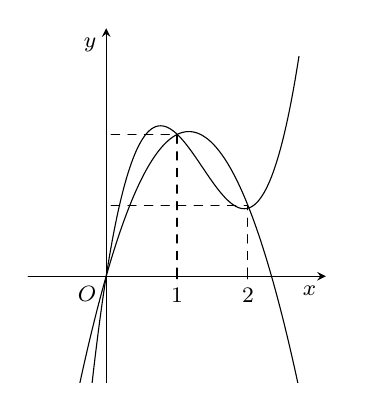
\begin{tikzpicture}[scale=.9, font=\footnotesize, line join=round, line cap=round, >=stealth]
			\draw[->] (-1.1,0)--(3.1,0) node[below left] {$x$};
			\draw[->] (0,-1.5)--(0,3.5) node[below left] {$y$};
			\draw (0,0) node [below left] {$O$};
			\foreach \x in {1,2}
			\draw[thin] (\x,1pt)--(\x,-1pt) node [below] {$\x$};
			\draw[dashed,thin](1,0)--(1,2)--(0,2);
			\draw[dashed,thin](2,0)--(2,1)--(0,1);
			\begin{scope}
				\clip (-1.1,-1.5) rectangle (3.5,3.1);
				\draw[samples=200,domain=-0.5:2.75,smooth,variable=\x] plot (\x,{-1.5*(\x)^2+3.5*(\x)+0});
				\draw[samples=200,domain=-0.5:2.75,smooth,variable=\x] plot (\x,{1.42*((\x)^3)+-5.785*((\x)^2)+6.37*(\x)+0});
			\end{scope}
		\end{tikzpicture}
	}
	\loigiai{
		Từ giả thuyết suy ra $f'(x)-g'(x)=ax(x-1)(x-2)=0 \Leftrightarrow \hoac{&x=0\\&x=1\\&x=2.}$\\
		Dựa vào đồ thị hàm số $f'(x)=ax^3+bx^2+cx+d$ ta thấy $a>0$.\\
		Do đó, $S_1=a\displaystyle\int\limits_0^2 \vert x(x-1)(x-2) \vert \mathrm{\,d}x=10 \Leftrightarrow a\cdot \dfrac{1}{2}=10 \Rightarrow a=20 \Rightarrow f'(x)-g'(x)=20(x^3-3x^2+2x)$.\\
		Khi đó, $f(x)-g(x)=\displaystyle\int\limits \left[f'(x)-g'(x)\right]\mathrm{\,d}x=20\displaystyle\int\limits (x^3-3x^2+2x)\mathrm{\,d}x=20\left(\dfrac{x^4}{4}-x^3+x^2\right) +C$.\\
		Mà $f(2)-g(2)=0 \Rightarrow f(2)-g(2)=20(4-8+4)+C=0 \Leftrightarrow C=0$.\\
		Suy ra $f(x)-g(x)=20\left(\dfrac{x^4}{4}-x^3+x^2\right)=5x^2(x^2-4x+4)=5x^2(x-2)^2$.
		Vậy $S=\displaystyle\int\limits_0^2 \left\vert 5x^2(x-2)^2 \right\vert \mathrm{\,d}x=\dfrac{16}{3}$.
	}
\end{ex}
\Closesolutionfile{ans}
\begin{indapan}{10}
	{ans/ans-2-TT-11-SGD-HungYen-23}
\end{indapan}


